\documentclass[conference]{IEEEtran}
\usepackage{amsmath,amssymb}
\usepackage{booktabs}
\usepackage{graphicx}
\usepackage{cite}
\usepackage{url}
\usepackage[hidelinks]{hyperref}
\title{QWeave: Correctness-First Deterministic and Learned Qubit Routing}
\author{\IEEEauthorblockN{Atharva Sheersh Pandey$^{1}$, Diptesh Das$^{1}$, Shrivardhini N$^{1}$, Haridasu Sreedhar$^{1}$, Prof. Bhuvaneswari M$^{2}$}
\IEEEauthorblockA{$^{1}$School of Computer Science and Engineering, VIT Vellore\\
$^{2}$Faculty Guide, School of Computer Science and Engineering, VIT Vellore\\
\{atharva.sheersh2024, diptesh.das2024, shrivardhini.n2024, haridasu.sreedhar2024\}@vitstudent.ac.in}}
\begin{document}
\maketitle
\begin{abstract}
Restricted two-qubit connectivity forces a compiler to place logical qubits
on physical sites and insert movement before nonlocal interactions. This paper
studies QWeave as a correctness-first compiler rather than treating low depth
alone as sufficient evidence. The deterministic path combines weighted initial
mapping, strict local improvement, and shortest-path SWAP routing; identity
mapping, Qiskit SABRE, and a small exact initial-mapping oracle are distinct
references. We prove termination of the finite mapping descent, preservation of
the routing layout invariant and supported unitary semantics, feasibility and
fixed-DAG optimality of the list scheduler, equivalence of directed-CNOT
lowering, and termination of the guarded learned route. These guarantees do not
prove policy quality. That question is evaluated on frozen benchmark v2:
180 synthetic cases, five final training seeds, and 792 held-out outputs.
Every tested output passed its applicable numerical semantic check and every
direction-lowered cost circuit passed ordered-coupler legality. The paired
GNN--PPO minus weighted depth difference was 0 gates with a 95\% bootstrap
interval of $[0,0]$; GNN--PPO and no-message-passing PPO also had paired median
depth and SWAP differences of 0. Training improved markedly on an untrained
policy, but the study supplies no evidence of a message-passing or
learned-routing advantage over the deterministic references.
The discrete SWAP-count probability distribution and an independent-error
success-probability proxy are also reported.  Weighted routing has the highest
median proxy value, $0.691$, while GNN--PPO and no-message PPO both have
$0.673$; these synthetic values are not measurements of hardware fidelity.
\end{abstract}
\begin{IEEEkeywords}
quantum compilation, qubit mapping, qubit routing, reinforcement learning, graph neural networks, scheduling
\end{IEEEkeywords}

\section{Introduction}
Quantum algorithms are commonly written with unrestricted two-qubit
interactions, whereas a device exposes a finite coupling graph. Compilation
must therefore choose an initial placement and transform every nonlocal
interaction into operations supported by that graph. Qiskit describes layout,
routing, translation, optimization, and scheduling as separate stages
\cite{ibmtranspiler}. SABRE uses bidirectional heuristic search for layout and
SWAP selection \cite{li2019sabre}; it is consequently a substantive baseline.

QWeave asks a narrower question: under a declared circuit language, topology,
mapping convention, and validation protocol, what do deterministic placement,
guarded learned routing, and post-routing scheduling each contribute? The
answer requires more than an edge-legality check. An emitted circuit can use
only valid couplers and still implement the wrong logical computation if a
layout update, source SWAP, parameter, or classical destination is mishandled.
For that reason, QWeave combines trace replay with numerical checks and keeps
mapping, routing, scheduling, and direction lowering as separately reported
stages.

This paper contributes (i) an explicit deterministic compiler and adapter
contract, (ii) formal correctness arguments for the invariants that can be
proved from that contract, (iii) a guarded GNN--PPO implementation with
message-passing and training controls, and (iv) a frozen held-out comparison
with paired uncertainty estimates and counterexamples. Learning-based routing
already exists \cite{pozzi2020rl,sinha2022gnn}; neither the use of PPO nor a
graph encoder is claimed as novel. The result is also deliberately bounded:
the tested policy does not outperform the weighted deterministic reference.

\section{Related Work}
NISQ compilation sits between abstract circuit descriptions and devices whose
connectivity, native gates, timing, and error characteristics constrain
execution. Standard references establish the computational model and the NISQ
setting, while Qiskit, OpenQL, and t|ket> illustrate retargetable compiler
stacks \cite{preskill2018nisq,bharti2022nisq,nielsenchuang2010,
javadiabhari2024qiskit,khammassi2021openql,sivarajah2020tket,
bandic2022fullstack}. QWeave follows this staged view and reports placement,
routing, lowering, and scheduling separately. Earlier compiler and instruction-
set work likewise separates high-level optimization from hardware-specific
execution, including scalable logical compilation, Quil, and eQASM
\cite{haener2018methodology,javadiabhari2015scaffcc,smith2016quil,
fu2019eqasm}.

Qubit mapping has been approached through compiler allocation, search, graph
methods, and local rewriting. Siraichi et al. formulate allocation directly;
Zulehner et al. use architecture-aware search; and Cowtan et al. and Childs et
al. study routing independently of a particular device
\cite{siraichi2018allocation,zulehner2019efficient,cowtan2019routing,
childs2019transformations}. Look-ahead nearest-neighbor optimization, exact
minimum-SWAP search, subgraph-isomorphism placement, commutation-aware
transformation, gate absorption, and topology-aware assignment further show
that routing cost depends on both circuit structure and the permitted rewrite
space \cite{wille2016lookahead,lye2015minimal,li2021subgraph,
itoko2020optimization,tan2021gateabsorption,steinberg2022topological}. SABRE's
bidirectional layout and heuristic SWAP search remains a substantive scalable
baseline \cite{li2019sabre,ibmsabre}.
Duration-aware remapping, noise-weighted allocation, SU(4)-specific compilation,
and MQT QMAP show why a single gate-count objective cannot represent every
target architecture \cite{deng2020codar,finigan2018allocation,
zulehner2019su4,wille2023qmap}.

Connectivity is only one hardware constraint. Noise-adaptive, variability-
aware, and error-aware compilers incorporate calibration information, while
timing-aware mappers and scheduling studies distinguish depth from duration
\cite{murali2019noise,tannu2019variability,nishio2020erroraware,
lao2022timing,guerreschi2018twostep}. Full-stack hardware studies and
teleportation-assisted mapping broaden the cost model beyond SWAP count
\cite{murali2019fullstack,hillmich2021teleportation}. QWeave's hardware-cost
study remains synthetic and therefore does not claim calibration-derived
fidelity. Crosstalk-aware compilation further demonstrates that parallelism,
frequency allocation, and correlated error can invalidate an independent-gate
model \cite{ding2020crosstalk,hua2022cqc}. Average gate fidelity and process
distance have precise channel-level definitions \cite{nielsen2002fidelity,
gilchrist2005distance}; randomized, direct, and cycle benchmarking estimate
device behavior under experimentally stated assumptions
\cite{magesan2012rb,wallman2016randomized,erhard2019cycle,
proctor2019direct,hashim2021randomized}. QWeave therefore calls its product of
declared gate-success terms a \emph{proxy}, not physical fidelity.

Scaling beyond a monolithic coupling graph introduces partitioning and
communication choices. Time-sliced partitioning, QUBO mapping for modular
architectures, Hamiltonian-simulation-specific compilation, and structured
design-space exploration expose tradeoffs between routing quality, latency,
and compiler runtime \cite{baker2020partitioning,bandic2023qubo,
laobrowne2021twoqan,bandic2020dse}. These methods motivate QWeave's explicit
topology and metric declarations, although the present experiments use only
connected single-device graphs.

Learning-based mapping includes reinforcement-learning policies, learned
initial layouts, and graph-guided search \cite{herbert2018rl,pozzi2020rl,
acampora2021neural,sinha2022gnn}. QWeave uses an edge-conditioned actor--critic
whose encoder draws on graph convolution and message passing, and whose update
uses PPO with generalized advantage estimation
\cite{kipf2017gcn,gilmer2017mpnn,schulman2017ppo,schulman2015gae}. Neither PPO
nor message passing is claimed as novel; the ablations test whether either
helps under the frozen protocol. GraphSAGE and graph attention provide broader
context for neighborhood aggregation, while Adam supplies the optimizer used
by many learned systems \cite{hamilton2017graphsage,velickovic2018gat,
kingma2015adam}. Because few-seed reinforcement-learning results are often
unstable, QWeave reports seed-level behavior, intervals, and controls following
the reproducibility concerns of Henderson et al. and Agarwal et al.
\cite{henderson2018drl,agarwal2021rliable}.

Exact optimization and automated planning provide reference solutions for
small instances. Integer programming can jointly model assignment and routing,
whereas temporal planning represents hardware actions and resource constraints
\cite{nannicini2022ip,venturelli2018temporal,venturelli2019reasoning}.
QWeave's CP-SAT component is intentionally smaller: it optimizes only a static
initial-mapping surrogate for at most eight logical qubits and therefore cannot
certify minimum SWAP count or routed depth.

Evaluation methodology also affects conclusions. Interaction-graph
characterization, randomized model circuits, volumetric benchmarks, holistic
stack benchmarks, SupermarQ, and QASMBench emphasize complementary notions of
scale, structure, capability, and application relevance
\cite{bandic2023characterization,cross2019volume,
blumekohout2020volumetric,mills2021holistic,tomesh2022supermarq,
li2020qasmbench}. QWeave consequently freezes circuit families, topologies,
seeds, validity checks, and paired statistics before interpreting method-level
differences. Application-oriented and hardware-agnostic benchmark frameworks
also distinguish result quality from scale and execution speed
\cite{lubinski2023benchmarks,martiel2021qscore,resch2022benchmarking}.


\section{Problem Formulation and Deterministic Path}
Let $C=(g_1,\ldots,g_T)$ be an ordered supported circuit on logical qubits
$L=\{0,\ldots,n-1\}$ and let $H=(P,E_H)$ be a connected undirected routing
graph. An initial mapping $m_0:L\rightarrow P$ is injective and uses the
convention $m(\mathrm{logical})=\mathrm{physical}$. The interaction graph
$G_C$ includes isolated logical qubits. An edge $(i,j)$ has weight $w_{ij}$
equal to its two-qubit interaction count. QWeave minimizes the placement
surrogate
{\large
\begin{equation}
 J(m)=\sum_{(i,j)\in E_C}w_{ij}\,d_H(m(i),m(j)),
 \label{eq:objective}
\end{equation}
}
where $d_H$ is shortest-path distance. Optional temporal decay replaces an
interaction count by $\delta^t$, but benchmark v2 uses integer counts.

The mapper places a high weighted-degree logical qubit on a high-centrality
physical node, then greedily assigns the remaining logical qubits using
interaction weight and partial distance cost. Deterministic ordering resolves
ties. Pairwise local search evaluates exchanges of occupied physical sites and
accepts the best exchange only when it strictly decreases $J$.

For each source operation, the deterministic router emits an adjacent
one- or two-qubit gate immediately. If a two-qubit gate is nonlocal, it selects
a deterministic shortest path and moves the first logical qubit toward the
second through edge-local SWAPs. Both forward and inverse layouts are updated
after every inserted SWAP. The Basic reference supplies identity mapping to
this router; weighted mapping supplies the greedy local-search layout. SABRE is
a separate Qiskit compiler path with a fixed seed.

The Qiskit adapter accepts unconditioned one- and two-qubit gates, one-qubit
resets, and a terminal measurement suffix while preserving global phase and
classical destinations. It rejects barriers, higher-arity gates, dynamic
control flow, and classically conditioned operations instead of silently
passing unsupported semantics. A trace records one event for each source gate
or inserted SWAP. Replay checks source order, parameters, targets, layout
updates, and the final mapping. SABRE receives both orientations of every
undirected routing edge so all methods share the same adjacency interpretation.

\section{Formal Correctness Arguments}
\begingroup\fontsize{11}{12.5}\selectfont
The propositions below cover algorithmic invariants under the stated input
contract. They do not establish that the static objective predicts minimum
route cost, that a learned policy is good, or that finite numerical probes are
a proof over all inputs.

Let $L$ and $P$ denote the logical and physical qubit sets, with
$|L|\leq |P|$. The routing graph $H=(P,E_H)$ is finite, simple, undirected,
and connected. The implementation enforces an injective layout
$m:L\rightarrow P$, the convention $m(\text{logical})=\text{physical}$,
contiguous physical labels, a supported gate family, positive declared
durations, and explicit random seeds. Directed coupling constraints are
handled only by the later lowering pass. These assumptions are necessary:
dropping connectivity removes the fallback guarantee, and accepting dynamic
control would require a different semantic argument.

\paragraph{Proposition 1 (mapping-search termination).}
The strict pair-exchange local search terminates after finitely many accepted
moves.

\paragraph{Proof.}
There are
{\large
\begin{equation}
 N_{\mathrm{map}}=\frac{|P|!}{(|P|-|L|)!}
 \label{eq:number-maps}
\end{equation}
}
injective maps from $L$ to $P$. Each accepted exchange changes the map and
strictly decreases $J$; hence a previously visited map cannot recur. The
number of accepted exchanges is at most $N_{\mathrm{map}}-1$, so the search
terminates. This proof also covers real-valued temporal weights because it
uses finiteness of the map set rather than integrality of $J$. The
implementation's iteration cap is an additional guard, not the basis of
termination.

\paragraph{Proposition 2 (layout and legality invariant).}
After every emitted operation, the forward layout remains injective, its
inverse agrees on occupied sites, and every emitted two-qubit operation uses an
edge of $E_H$.

\paragraph{Proof.}
The claim holds initially by the mapping contract. An inserted SWAP exchanges
the logical occupants of two adjacent physical sites; updating both maps by
the same transposition preserves injectivity and inverse agreement. A source
one-qubit gate cannot violate edge legality. A source two-qubit gate is emitted
only when its current images are adjacent, either immediately or after the
shortest-path swaps. Induction over the emitted sequence proves the claim.

\paragraph{Lemma 1 (masked-policy legality).}
Let $A$ be the finite action set and $A_{\mathrm{legal}}(s)\neq\varnothing$
the actions permitted in state $s$. If $z_\theta(s,a)$ is the actor logit, set
$Z_\theta(s)=\sum_{b\in A_{\mathrm{legal}}(s)}\exp z_\theta(s,b)$. The masked
policy is
\begin{equation}
 \pi_\theta(a\mid s)=
 \begin{cases}
 \displaystyle\frac{\exp z_\theta(s,a)}{Z_\theta(s)},
 &a\in A_{\mathrm{legal}}(s),\\[5pt]
 0,&a\notin A_{\mathrm{legal}}(s).
 \end{cases}
 \label{eq:masked-policy}
\end{equation}
Therefore illegal actions have zero probability and legal probabilities sum
to one.

\paragraph{Proof.}
Every exponential in the denominator is positive, so the denominator is
strictly positive. The definition assigns zero outside the legal set. Summing
the first branch over the legal set returns the denominator divided by itself.
The implementation realizes the zero branch by masking logits before softmax;
property tests check exact zero for illegal entries and unit normalization.

\paragraph{Theorem 1 (supported unitary semantics).}
For an equal-width circuit containing only supported unitary one- and
two-qubit gates, let $R_k$ be the physical route after the first $k$
source gates, let $C_k$ be the corresponding logical prefix, and let $m_k$
be the current layout. With $P_m$ denoting the wire
permutation induced by $m$,
{\large
\begin{equation}
 U_{R_k}P_{m_0}=P_{m_k}U_{C_k}
 \quad\text{for }0\leq k\leq T .
 \label{eq:route-invariant}
\end{equation}
}

\paragraph{Proof.}
At $k=0$ both prefixes are identities, so the equality holds. Assume it holds
through source gate $k$. For a physical transposition $\tau=(u\ v)$ and its
SWAP unitary $S_{uv}$,
{\large
\begin{equation}
 S_{uv}P_m=P_{\tau\circ m}.
 \label{eq:swap-permutation}
\end{equation}
}
Thus an inserted physical SWAP and the corresponding layout update change only
the representation of the logical state. Once the operands of logical gate
$g_{k+1}$ are adjacent, its physical realization $\widetilde g_{k+1}$ obeys
$\widetilde g_{k+1}P_m=P_m g_{k+1}$. Repeated use of
Equation~\eqref{eq:swap-permutation}, followed by this gate identity and the
induction hypothesis, yields
$U_{R_{k+1}}P_{m_0}=P_{m_{k+1}}U_{C_{k+1}}$. At $k=T$, the final routed
unitary equals the logical unitary up to the declared initial and final
permutations. Global phase is copied by the adapter, so equality is interpreted
under the same phase convention used by the numerical checker.

\paragraph{Proposition 3 (fixed-route scheduling).}
For positive operation durations and no resource constraints beyond physical
qubit exclusivity, the list scheduler returns a feasible schedule. Its
makespan equals the weighted critical-path length of the fixed per-qubit
precedence DAG and is therefore minimal among schedules that preserve that DAG.

\paragraph{Proof.}
The DAG contains an edge between successive operations on each physical qubit.
Every edge points from an earlier routed operation to a later one, so a cycle
would imply a strictly increasing sequence of indices returning to its start;
the graph is acyclic. Consequently, incomparable ready operations share no
qubit and may overlap.
For operation $i$, the scheduler uses
{\large
\begin{equation}
 r_i=d_i+\max_{j\in\mathrm{succ}(i)}r_j,
 \qquad
 s_i=\max_{j\in\mathrm{pred}(i)}(s_j+d_j),
 \label{eq:schedule}
\end{equation}
}
with an empty maximum equal to zero. Thus each operation starts after every
predecessor finishes, proving feasibility. Every schedule respecting the DAG
has makespan at least
{\large
\begin{equation}
 \mathrm{LB}=\max\!\left\{
 \max_{\rho\in\mathcal P(D)}\sum_{i\in\rho}d_i,
 \max_{q\in P}\sum_{i:q\in Q_i}d_i
 \right\},
 \label{eq:schedule-lower-bound}
\end{equation}
}
where $\mathcal P(D)$ is the set of DAG paths and $Q_i$ the qubits used by
operation $i$. The per-qubit load is itself represented by a precedence chain,
and earliest-start recursion attains the weighted critical-path bound. The
returned makespan is therefore optimal for this fixed DAG and resource model.
This statement does not allow gate commutation or model control electronics.

\paragraph{Proposition 4 (directed lowering).}
If at least one orientation of an undirected routing edge supports CNOT, the
lowering pass implements either requested CNOT orientation and an edge-local
SWAP using only declared directed CNOTs and one-qubit Hadamards.

\paragraph{Proof.}
For a supported physical CNOT directed from $v$ to $u$, the opposite
orientation satisfies
{\large
\begin{equation}
 \mathrm{CX}_{u\rightarrow v}
 =(H_u\otimes H_v)\,
 \mathrm{CX}_{v\rightarrow u}\,
 (H_u\otimes H_v).
 \label{eq:reverse-cx}
\end{equation}
}
An undirected SWAP is three alternating CNOTs. Replacing each unavailable
orientation by Equation~\eqref{eq:reverse-cx} preserves the product unitary
and leaves every two-qubit instruction on an allowed ordered arc.

\paragraph{Proposition 5 (guarded-route termination).}
For a finite supported circuit on a finite connected routing graph, the
guarded learned environment terminates and returns a legal route.

\paragraph{Proof.}
Each policy-controlled segment has a finite step limit. On repeated
nonprogress or exhaustion, fallback selects a finite shortest path, performs
adjacent swaps, and executes the current gate. Hence fallback advances the
source index. If the guard permits at most $B$ policy actions per pending gate,
then a shortest path in a connected $|P|$-vertex graph has at most $|P|-1$
edges and needs at most $|P|-2$ SWAPs to make two operands adjacent. For $T$
source operations, the number of policy, fallback-SWAP, and execute actions is
therefore bounded above by $T(B+|P|-1)$. Proposition 2 gives legality for every
fallback operation, and replay validation must succeed before the environment
returns a result.

\paragraph{Proposition 6 (monotonic independent-error proxy).}
For a lowered route $R$ with declared independent gate-error probabilities
$0\leq\epsilon_g<1$, define
{\large
\begin{equation}
 \widehat F(R)=\prod_{g\in R}(1-\epsilon_g)
 =\exp\!\left(\sum_{g\in R}\log(1-\epsilon_g)\right).
 \label{eq:fidelity-proxy}
\end{equation}
}
Appending any nonzero-error gate cannot increase $\widehat F$. Under a
homogeneous two-qubit error $\epsilon_2$, one additional SWAP lowered to three
CNOTs multiplies the proxy by $(1-\epsilon_2)^3$ before any extra one-qubit
direction-reversal cost.

\paragraph{Proof.}
Each factor lies in $(0,1]$, so multiplying by another factor cannot increase
the product. A SWAP contributes three CNOT factors, giving the stated ratio.
Taking logarithms converts the product into the additive quantity used for
paired statistics. This is an exact statement about the declared independent-
error model; correlated noise, drift, crosstalk, leakage, and calibration
uncertainty are absent, so $\widehat F$ is not physical state, process, or gate
fidelity \cite{nielsen2002fidelity,gilchrist2005distance}.

\endgroup
\section{Learned Router}
The Gymnasium environment exposes an \textsc{Execute} action and one SWAP
action for every sorted hardware edge. Its observation contains five features
per physical node, four per hardware edge, a five-value frontier description,
the current logical-to-physical mapping, and a binary legal-action mask.
Illegal actions do not mutate the circuit or layout. Fallback counts are
reported because the termination guard can conceal a weak policy.

The actor--critic performs two rounds of edge-conditioned message passing and
scores every edge SWAP plus \textsc{Execute}. PPO uses clipped policy ratios,
generalized advantage estimation, value and entropy terms, and gradient
clipping \cite{schulman2017ppo,schulman2015gae}. A zero-message-passing PPO
control preserves the optimizer and reward, while an untrained graph control
preserves the architecture without PPO updates. All variants start from the
weighted deterministic map, making this a routing-policy comparison rather
than a learned-layout experiment.

\section{Validation and Experimental Protocol}
Structural replay checks mapping completeness, injectivity, source-gate order,
inserted SWAP consistency, global phase, and edge legality. For equal-width
unitary circuits of at most six qubits, QWeave evaluates
Equation~\eqref{eq:route-invariant} at $k=T$ as an exact operator equality.
Wider unitary circuits and outputs with idle physical sites use reproducible
layout-aware statevector probes up to 12 physical qubits. Exact equality is a
semantic proof for the evaluated circuit; a finite probe set is evidence that
can detect faults but is not a universal proof. Reset and terminal-measurement
circuits receive structural replay. Branch-dependent dynamic control remains
unsupported.

After routing, the fixed-route scheduler measures depth or declared-duration
makespan on the same legal route. A separate hardware-cost pass lowers CNOTs
and SWAPs to declared directed couplers, validates ordered arcs, then evaluates
the schedule and an independent-error proxy. Durations and edge errors are
synthetic assumptions rather than device calibrations.

The requested ``probability density'' is treated according to the data type.
SWAP count $S_m$ is discrete, so the estimand is an empirical probability mass
function rather than a continuous density. After collapsing seeds within each
held-out case,
\begin{equation}
 \begin{aligned}
 \widehat p_m(s)&=\frac{1}{N}\sum_{i=1}^{N}
 \mathbf 1\!\left[S_{m,i}=s\right],\\
 \widehat P_m(S\leq s)&=\sum_{u\leq s}\widehat p_m(u).
 \end{aligned}
 \label{eq:swap-pmf}
\end{equation}
The mass sums to one because each of the $N=36$ cases contributes to exactly
one SWAP-count bin. We plot the empirical cumulative distribution, which avoids
introducing a kernel bandwidth for a small discrete sample. Fidelity is kept
separate: Equation~\eqref{eq:fidelity-proxy} is evaluated only after directed
lowering, using the declared synthetic error profile.

Benchmark version 2.0 freezes 180 cases at four, six, and eight logical
qubits, with two instances per family. Sixty training cases use GHZ,
layered-CX, seeded-interaction, Bernstein--Vazirani, and QAOA MaxCut families;
the latter follows the alternating-operator construction of
Farhi et al.~\cite{farhi2014qaoa}. Eighty-four validation cases test topology transfer and
held-out families. The 36 untouched test cases combine QFT circuits, motivated
by the approximate transform of Coppersmith~\cite{coppersmith2002qft}, and
hardware-efficient circuits with two-row grids, chorded rings, and larger
grids containing idle sites. Every case stores QASM, source hash, undirected
and directed edges, and declared synthetic error values.

Three candidates receive 1,024 training steps and validation seed 101. The
selection score is median depth plus half the SWAP count plus five times the
fallback count. The selected candidate is trained for 4,096 steps at seeds 7,
17, 29, 41, and 53 for both GNN--PPO and the no-message control. The untrained
control uses the same initialization seeds. SABRE uses the same five seeds;
Basic and weighted routing are deterministic. Runtime is the median of three
measurements after one warmup. Seeds are collapsed within each case before
paired differences are formed. Confidence intervals use 5,000 deterministic
bootstrap resamples with seed 20260921.

\section{Results}
The immutable benchmark was produced under Python 3.11.15 and Qiskit 2.5.2;
its documented clean-clone run passed the then-current 69-test suite. The live
GitHub head later passed an integrated 104-test suite after CLI and web
additions. This later test count verifies the expanded software surface but
does not replace or rerun the 792-record benchmark. The aggressive validation
candidate scored 19.5; conservative and standard each scored 24.0.
Table~\ref{tab:test-results} summarizes the 36 held-out cases.
For seeded methods, each case contributes its within-case seed median. All 792
outputs passed their applicable numerical check. QWeave routes also passed
symbolic replay; SABRE has no QWeave trace. Every unit-duration scheduling
delta was zero, as expected when circuit depth already expresses the same
per-qubit precedence.

\begin{figure*}[t]
\centering
\includegraphics[width=0.94\textwidth]{../../../results/benchmark_v2/figures/method_medians.png}
\caption{Held-out median depth and SWAP count after seed collapse. The graph
shows aggregate routing cost; it does not encode uncertainty or device noise.}
\label{fig:method-medians}
\end{figure*}

\begin{table*}[t]
\centering
\caption{Benchmark-v2 test summary. Runtime is median wall time in seconds.}
\label{tab:test-results}
\small
\begin{tabular}{lrrrr}
\toprule
Method & Depth & SWAP & Runtime & Fallback \\
\midrule
Basic & 48.5 & 11.5 & 0.0022 & 0 \\
Weighted & 36.0 & 0.0 & 0.0036 & 0 \\
SABRE & 46.0 & 7.0 & 0.0028 & 0 \\
GNN--PPO & 37.5 & 0.0 & 0.3473 & 4543 \\
No-message PPO & 36.0 & 0.0 & 0.1040 & 742 \\
Untrained GNN & 198.0 & 193.0 & 0.6681 & 8059 \\
\bottomrule
\end{tabular}
\end{table*}

The paired GNN--PPO minus weighted depth difference was 0 gates with interval
$[0,0]$; versus SABRE it was 0 with interval $[0,5]$. Its paired SWAP
difference versus weighted routing was 0 with interval $[0,5]$. GNN--PPO and
no-message PPO had paired median depth and SWAP differences of 0 with
intervals $[0,0]$, so the experiment supplies no evidence that message passing
helped. Training did matter relative to the untrained GNN: the paired depth
difference was $-162.5$ with interval $[-184,-106]$, and the SWAP difference
was $-175$ with interval $[-223,-148]$.

Family results explain the aggregate. On hardware-efficient circuits,
weighted, GNN--PPO, and no-message PPO all had median depth 27 and no SWAPs. On
QFT, weighted routing had median depth 71.5 and 16.5 SWAPs, GNN--PPO had 83.5
and 41, and no-message PPO had 90 and 31.5. GNN--PPO improved by eight depth
layers on \texttt{qft\_i1\_6q\_chorded\_ring}, but regressed by 89 layers
and 130 SWAPs on \texttt{qft\_i1\_8q\_grid2}. It invoked 4,543 test
fallbacks, compared with 742 for no-message PPO and zero for deterministic
methods. Seed 29 was unstable, ending with 212 training fallbacks and a recent
mean return near $-103$.

\subsection{SWAP Probability and Fidelity Proxy}
Table~\ref{tab:swap-fidelity} and Fig.~\ref{fig:swap-fidelity} focus on the two
requested metrics. Because SWAP count is discrete, the left panel is an
empirical distribution rather than a continuous probability density. Weighted,
GNN--PPO, and no-message PPO each produced a zero-SWAP within-case median on
20 of 36 cases ($0.556$ probability mass). Their upper tails differ: the
learned policies incurred larger QFT regressions, and the untrained control was
far outside the trained and deterministic distributions.

\begin{table}[t]
\centering
\caption{Discrete zero-SWAP mass and synthetic fidelity proxy.}
\label{tab:swap-fidelity}
\small
\resizebox{\columnwidth}{!}{%
\begin{tabular}{lrrr}
\toprule
Method & $\widehat P(S=0)$ & Median $\widehat F$ & $\widehat F$ IQR \\
\midrule
Basic & 0.222 & 0.526 & [0.294, 0.704] \\
Weighted & 0.556 & 0.691 & [0.343, 0.787] \\
SABRE & 0.222 & 0.569 & [0.387, 0.741] \\
GNN--PPO & 0.556 & 0.673 & [0.204, 0.787] \\
No-message PPO & 0.556 & 0.673 & [0.238, 0.787] \\
Untrained GNN & 0.000 & 0.0026 & [$1.29\!\times\!10^{-5}$, 0.024] \\
\bottomrule
\end{tabular}
}
\end{table}

\begin{figure*}[t]
\centering
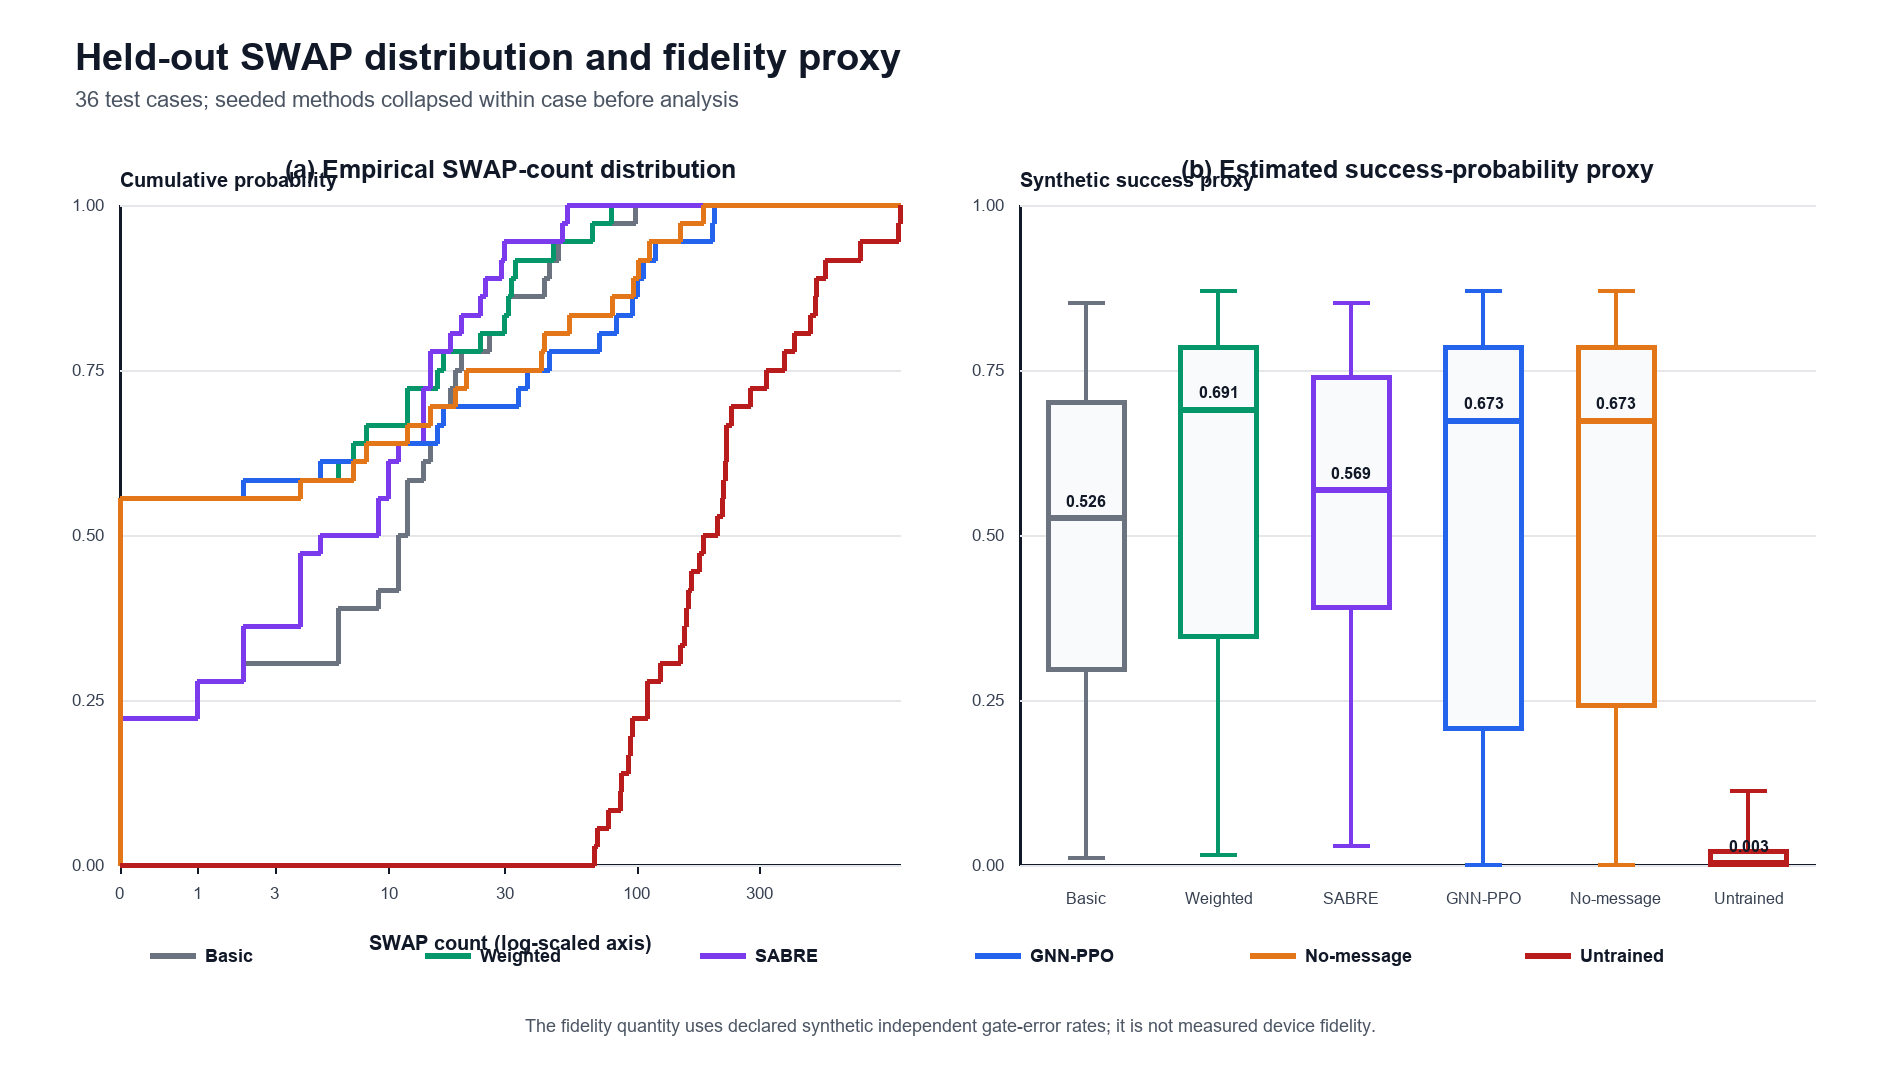
\includegraphics[width=0.96\textwidth]{../assets/swap_fidelity_distributions.png}
\caption{Left: empirical cumulative probability of case-level SWAP count on a
log-scaled horizontal axis. Right: case-level distribution of the declared
independent-error success proxy after directed lowering. Boxes show IQRs,
center lines show medians, and whiskers show minima and maxima. The right panel
is not measured hardware fidelity.}
\label{fig:swap-fidelity}
\end{figure*}

The paired GNN--PPO minus weighted log-proxy difference was 0 with a 95\%
bootstrap interval $[-0.171,0]$; GNN--PPO minus no-message PPO was
$0\,[0,0]$. Thus the proxy supplies no learned or message-passing advantage.
GNN--PPO did improve strongly over the untrained graph control: the paired
log-proxy difference was $5.274\,[4.480,6.458]$. Weighted routing had the
largest median proxy, $0.691$, but this ranking is conditional on the declared
synthetic independent-error profile. Real fidelity would require calibration-
derived channels or device executions and an explicit estimator
\cite{magesan2012rb,erhard2019cycle,lubinski2023benchmarks}.

\begin{figure*}[t]
\centering
\includegraphics[width=0.94\textwidth]{../../../results/benchmark_v2/figures/learning_curves.png}
\caption{Five-seed learning curves. Lines show the median recent episode
return and bands show the interquartile range. Neither curve is monotone, and
the GNN curve degrades more strongly late in training.}
\label{fig:learning-curves}
\end{figure*}

Before direction lowering, most routes were illegal on the one-way couplers.
After reverse-CNOT and SWAP synthesis, all 792 cost circuits passed ordered-arc
legality. Median added depth was 32 for weighted routing, 34 for SABRE, 37.5
for GNN--PPO, 28.5 for no-message PPO, 57 for Basic, and 441 for the untrained
GNN. The corrected paired GNN--PPO minus weighted makespan difference was
0 ns with interval $[0,1113]$. These synthetic proxy costs provide no learned
advantage.

\section{Threats to Validity}
The formal results depend on the supported gate contract, a connected routing
graph, correct primitive gate implementations, and the absence of unmodelled
shared hardware resources. They prove preservation properties of the
algorithms, not software free of defects; tests and independent reruns address
implementation risk. Numerical probes for wider circuits are incomplete by
construction. Measurement, reset, and dynamic-control semantics do not receive
the same exact unitary argument.

The empirical study uses synthetic circuits, durations, and error rates. Its
five seeds and 36 held-out cases support paired statements about benchmark v2,
not general performance or state-of-the-art rank. Runtime is machine-specific,
and fallback makes the learned methods safe while also weakening the
interpretation of policy-only behavior. The retained pre-correction record is
disclosed because its duration fields scheduled pre-lowering circuits; the
schema-2.1 replay recomputed only direction-dependent cost fields from saved
checkpoints and frozen cases.

The empirical SWAP curve is a distribution over 36 generated test cases, not a
probability law for unseen circuits. The success proxy assumes independent
gate failures and multiplies declared scalar error terms. It is useful for
explaining why extra lowered SWAPs normally reduce predicted success, but it
cannot represent coherent error, crosstalk, leakage, drift, readout mitigation,
or uncertainty in calibration. Calling it measured fidelity would therefore
be incorrect \cite{wallman2016randomized,hashim2021randomized,
resch2022benchmarking}.

\section{Conclusion}
QWeave combines an explicit deterministic reference, a small mapping oracle,
fixed-route scheduling, directed lowering, and a guarded learned router.
Formal arguments now state why strict mapping descent terminates, why routing
preserves the declared layout semantics, why the fixed-DAG scheduler is
feasible and makespan-optimal under its model, why direction reversal is
unitarily sound, and why fallback terminates. Benchmark v2 complements those
proofs with held-out evidence. PPO training clearly improves on an untrained
policy, but the tested message-passing component and learned route do not
improve on weighted routing. The SWAP probability distribution and synthetic
success proxy reach the same bounded conclusion: weighted routing has the
highest median proxy, while GNN--PPO and its no-message control are tied in
paired median log success. Larger preregistered, device-derived studies are
needed before any superiority or calibrated-fidelity claim.

\begin{thebibliography}{00}
\bibitem{ibmtranspiler} IBM Quantum, "Transpiler stages," IBM Quantum Documentation, 2026.
\bibitem{li2019sabre} G. Li, Y. Ding, and Y. Xie, "Tackling the qubit mapping problem for NISQ-era quantum devices," in Proc. ASPLOS, 2019.
\bibitem{pozzi2020rl} M. G. Pozzi, S. J. Herbert, A. Sengupta, and R. D. Mullins, "Using reinforcement learning to perform qubit routing in quantum compilers," arXiv:2007.15957, 2020.
\bibitem{sinha2022gnn} A. Sinha, U. Azad, and H. Singh, "Qubit routing using graph neural network aided Monte Carlo tree search," in Proc. AAAI, 2022.
\bibitem{preskill2018nisq} J. Preskill, "Quantum computing in the NISQ era and beyond," Quantum, vol. 2, p. 79, 2018.
\bibitem{bharti2022nisq} K. Bharti et al., "Noisy intermediate-scale quantum algorithms," Rev. Mod. Phys., vol. 94, no. 1, p. 015004, 2022.
\bibitem{nielsenchuang2010} M. A. Nielsen and I. L. Chuang, Quantum Computation and Quantum Information, 10th anniversary ed. Cambridge, U.K.: Cambridge Univ. Press, 2010.
\bibitem{javadiabhari2024qiskit} A. Javadi-Abhari et al., "Quantum computing with Qiskit," arXiv:2405.08810, 2024.
\bibitem{khammassi2021openql} N. Khammassi et al., "OpenQL: A portable quantum programming framework for quantum accelerators," ACM J. Emerg. Technol. Comput. Syst., vol. 18, no. 1, pp. 1-24, 2021.
\bibitem{sivarajah2020tket} S. Sivarajah, S. Dilkes, A. Cowtan, W. Simmons, A. Edgington, and R. Duncan, "t|ket>: A retargetable compiler for NISQ devices," Quantum Sci. Technol., vol. 6, no. 1, p. 014003, 2020.
\bibitem{bandic2022fullstack} M. Bandic, S. Feld, and C. G. Almudever, "Full-stack quantum computing systems in the NISQ era: Algorithm-driven and hardware-aware compilation techniques," in Proc. DATE, pp. 1-6, 2022.
\bibitem{siraichi2018allocation} M. Y. Siraichi, V. F. dos Santos, S. Collange, and F. M. Q. Pereira, "Qubit allocation," in Proc. CGO, pp. 113-125, 2018.
\bibitem{zulehner2019efficient} A. Zulehner, A. Paler, and R. Wille, "An efficient methodology for mapping quantum circuits to the IBM QX architectures," IEEE Trans. Comput.-Aided Design Integr. Circuits Syst., vol. 38, no. 7, pp. 1226-1236, 2019.
\bibitem{cowtan2019routing} A. Cowtan, S. Dilkes, R. Duncan, A. Krajenbrink, W. Simmons, and S. Sivarajah, "On the qubit routing problem," in Proc. TQC, LIPIcs, vol. 135, pp. 5:1-5:32, 2019.
\bibitem{childs2019transformations} A. M. Childs, E. Schoute, and C. M. Unsal, "Circuit transformations for quantum architectures," in Proc. TQC, LIPIcs, vol. 135, pp. 3:1-3:24, 2019.
\bibitem{wille2016lookahead} R. Wille, O. Keszocze, M. Walter, P. Rohrs, A. Chattopadhyay, and R. Drechsler, "Look-ahead schemes for nearest neighbor optimization of 1D and 2D quantum circuits," in Proc. ASP-DAC, pp. 292-297, 2016.
\bibitem{lye2015minimal} A. Lye, R. Wille, and R. Drechsler, "Determining the minimal number of SWAP gates for multi-dimensional nearest neighbor quantum circuits," in Proc. ASP-DAC, pp. 178-183, 2015.
\bibitem{li2021subgraph} S. Li, X. Zhou, and Y. Feng, "Qubit mapping based on subgraph isomorphism and filtered depth-limited search," IEEE Trans. Comput., vol. 70, no. 11, pp. 1777-1788, 2021.
\bibitem{itoko2020optimization} T. Itoko, R. Raymond, T. Imamichi, and A. Matsuo, "Optimization of quantum circuit mapping using gate transformation and commutation," Integration, vol. 70, pp. 43-50, 2020.
\bibitem{tan2021gateabsorption} B. Tan and J. Cong, "Optimal qubit mapping with simultaneous gate absorption," arXiv:2109.06445, 2021.
\bibitem{steinberg2022topological} M. A. Steinberg, S. Feld, C. G. Almudever, M. Marthaler, and J.-M. Reiner, "Topological-graph dependencies and scaling properties of a heuristic qubit-assignment algorithm," IEEE Trans. Quantum Eng., vol. 3, pp. 1-14, 2022.
\bibitem{ibmsabre} IBM Quantum, "SabreLayout API reference," IBM Quantum Documentation, 2026.
\bibitem{murali2019noise} P. Murali, J. M. Baker, A. Javadi-Abhari, F. T. Chong, and M. Martonosi, "Noise-adaptive compiler mappings for noisy intermediate-scale quantum computers," in Proc. ASPLOS, pp. 1015-1029, 2019.
\bibitem{tannu2019variability} S. S. Tannu and M. K. Qureshi, "Not all qubits are created equal: A case for variability-aware policies for NISQ-era quantum computers," in Proc. ASPLOS, pp. 987-999, 2019.
\bibitem{nishio2020erroraware} S. Nishio, Y. Pan, T. Satoh, H. Amano, and R. Van Meter, "Extracting success from IBM's 20-qubit machines using error-aware compilation," ACM J. Emerg. Technol. Comput. Syst., vol. 16, no. 3, pp. 1-25, 2020.
\bibitem{lao2022timing} L. Lao, H. van Someren, I. Ashraf, and C. G. Almudever, "Timing and resource-aware mapping of quantum circuits to superconducting processors," IEEE Trans. Comput.-Aided Design Integr. Circuits Syst., vol. 41, no. 2, pp. 359-371, 2022.
\bibitem{guerreschi2018twostep} G. G. Guerreschi and J. Park, "Two-step approach to scheduling quantum circuits," Quantum Sci. Technol., vol. 3, no. 4, p. 045003, 2018.
\bibitem{murali2019fullstack} P. Murali et al., "Full-stack, real-system quantum computer studies: Architectural comparisons and design insights," in Proc. ISCA, pp. 527-540, 2019.
\bibitem{hillmich2021teleportation} S. Hillmich, A. Zulehner, and R. Wille, "Exploiting quantum teleportation in quantum circuit mapping," in Proc. ASP-DAC, pp. 792-797, 2021.
\bibitem{baker2020partitioning} J. M. Baker, C. Duckering, A. Hoover, and F. T. Chong, "Time-sliced quantum circuit partitioning for modular architectures," in Proc. Computing Frontiers, pp. 98-107, 2020.
\bibitem{bandic2023qubo} M. Bandic et al., "Mapping quantum circuits to modular architectures with QUBO," arXiv:2305.06687, 2023.
\bibitem{laobrowne2021twoqan} L. Lao and D. E. Browne, "2QAN: A quantum compiler for 2-local qubit Hamiltonian simulation algorithms," arXiv:2108.02099, 2021.
\bibitem{bandic2020dse} M. Bandic, H. Zarein, E. Alarcon, and C. G. Almudever, "On structured design space exploration for mapping of quantum algorithms," in Proc. DCIS, pp. 1-6, 2020.
\bibitem{herbert2018rl} S. Herbert and A. Sengupta, "Using reinforcement learning to find efficient qubit routing policies for deployment in near-term quantum computers," arXiv:1812.11619, 2018.
\bibitem{acampora2021neural} G. Acampora and R. Schiattarella, "Deep neural networks for quantum circuit mapping," Neural Comput. Appl., vol. 33, pp. 13723-13743, 2021.
\bibitem{kipf2017gcn} T. N. Kipf and M. Welling, "Semi-supervised classification with graph convolutional networks," in Proc. ICLR, 2017.
\bibitem{gilmer2017mpnn} J. Gilmer, S. S. Schoenholz, P. F. Riley, O. Vinyals, and G. E. Dahl, "Neural message passing for quantum chemistry," in Proc. ICML, PMLR, vol. 70, pp. 1263-1272, 2017.
\bibitem{schulman2017ppo} J. Schulman, F. Wolski, P. Dhariwal, A. Radford, and O. Klimov, "Proximal policy optimization algorithms," arXiv:1707.06347, 2017.
\bibitem{schulman2015gae} J. Schulman, P. Moritz, S. Levine, M. I. Jordan, and P. Abbeel, "High-dimensional continuous control using generalized advantage estimation," arXiv:1506.02438, 2015.
\bibitem{nannicini2022ip} G. Nannicini, L. S. Bishop, O. Gunluk, and P. Jurcevic, "Optimal qubit assignment and routing via integer programming," ACM Trans. Quantum Comput., vol. 4, no. 1, 2022.
\bibitem{venturelli2018temporal} D. Venturelli, M. Do, E. Rieffel, and J. Frank, "Compiling quantum circuits to realistic hardware architectures using temporal planners," Quantum Sci. Technol., vol. 3, no. 2, p. 025004, 2018.
\bibitem{venturelli2019reasoning} D. Venturelli et al., "Quantum circuit compilation: An emerging application for automated reasoning," in Proc. SPARK, 2019.
\bibitem{bandic2023characterization} M. Bandic, C. G. Almudever, and S. Feld, "Interaction graph-based characterization of quantum benchmarks for improving quantum circuit mapping techniques," Quantum Mach. Intell., vol. 5, p. 40, 2023.
\bibitem{cross2019volume} A. W. Cross, L. S. Bishop, S. Sheldon, P. D. Nation, and J. M. Gambetta, "Validating quantum computers using randomized model circuits," Phys. Rev. A, vol. 100, p. 032328, 2019.
\bibitem{blumekohout2020volumetric} R. Blume-Kohout and K. C. Young, "A volumetric framework for quantum computer benchmarks," Quantum, vol. 4, p. 362, 2020.
\bibitem{mills2021holistic} D. Mills, S. Sivarajah, T. L. Scholten, and R. Duncan, "Application-motivated, holistic benchmarking of a full quantum computing stack," Quantum, vol. 5, p. 415, 2021.
\bibitem{tomesh2022supermarq} T. Tomesh et al., "SupermarQ: A scalable quantum benchmark suite," in Proc. HPCA, pp. 587-603, 2022.
\bibitem{li2020qasmbench} A. Li and S. Krishnamoorthy, "QASMBench: A low-level QASM benchmark suite for NISQ evaluation and simulation," arXiv:2005.13018, 2020.
\bibitem{farhi2014qaoa} E. Farhi, J. Goldstone, and S. Gutmann, "A quantum approximate optimization algorithm," arXiv:1411.4028, 2014.
\bibitem{coppersmith2002qft} D. Coppersmith, "An approximate Fourier transform useful in quantum factoring," arXiv:quant-ph/0201067, 2002.
\bibitem{haener2018methodology} T. H\"aner, D. S. Steiger, K. Svore, and M. Troyer, "A software methodology for compiling quantum programs," \emph{Quantum Sci. Technol.}, vol. 3, no. 2, p. 020501, 2018. PDF: \url{https://arxiv.org/pdf/1604.01401}.
\bibitem{javadiabhari2015scaffcc} A. JavadiAbhari et al., "ScaffCC: Scalable compilation and analysis of quantum programs," \emph{Parallel Comput.}, vol. 45, pp. 2--17, 2015. PDF: \url{https://arxiv.org/pdf/1507.01902}.
\bibitem{smith2016quil} R. S. Smith, M. J. Curtis, and W. J. Zeng, "A practical quantum instruction set architecture," arXiv:1608.03355, 2016. PDF: \url{https://arxiv.org/pdf/1608.03355}.
\bibitem{fu2019eqasm} X. Fu et al., "eQASM: An executable quantum instruction set architecture," in \emph{Proc. MICRO}, pp. 224--237, 2019. PDF: \url{https://arxiv.org/pdf/1808.02449}.
\bibitem{deng2020codar} H. Deng, Y. Zhang, and Q. Li, "CODAR: A contextual duration-aware qubit mapping for various NISQ devices," arXiv:2002.10915, 2020. PDF: \url{https://arxiv.org/pdf/2002.10915}.
\bibitem{ding2020crosstalk} Y. Ding, P. Gokhale, S. F. Lin, R. Rines, T. Propson, and F. T. Chong, "Systematic crosstalk mitigation for superconducting qubits via frequency-aware compilation," in \emph{Proc. MICRO}, 2020. PDF: \url{https://arxiv.org/pdf/2008.09503}.
\bibitem{finigan2018allocation} W. Finigan, M. Cubeddu, T. Lively, J. Flick, and P. Narang, "Qubit allocation for noisy intermediate-scale quantum computers," arXiv:1810.08291, 2018. PDF: \url{https://arxiv.org/pdf/1810.08291}.
\bibitem{zulehner2019su4} A. Zulehner and R. Wille, "Compiling SU(4) quantum circuits to IBM QX architectures," in \emph{Proc. ASP-DAC}, pp. 185--190, 2019. PDF: \url{https://arxiv.org/pdf/1808.05661}.
\bibitem{wille2023qmap} R. Wille and L. Burgholzer, "MQT QMAP: Efficient quantum circuit mapping," in \emph{Proc. ISPD}, pp. 198--204, 2023. PDF: \url{https://arxiv.org/pdf/2301.11935}.
\bibitem{hua2022cqc} F. Hua et al., "A synergistic compilation workflow for tackling crosstalk in quantum machines," arXiv:2207.05751, 2022. PDF: \url{https://arxiv.org/pdf/2207.05751}.
\bibitem{nielsen2002fidelity} M. A. Nielsen, "A simple formula for the average gate fidelity of a quantum dynamical operation," \emph{Phys. Lett. A}, vol. 303, no. 4, pp. 249--252, 2002. PDF: \url{https://arxiv.org/pdf/quant-ph/0205035}.
\bibitem{gilchrist2005distance} A. Gilchrist, N. K. Langford, and M. A. Nielsen, "Distance measures to compare real and ideal quantum processes," \emph{Phys. Rev. A}, vol. 71, p. 062310, 2005. PDF: \url{https://arxiv.org/pdf/quant-ph/0408063}.
\bibitem{magesan2012rb} E. Magesan, J. M. Gambetta, and J. Emerson, "Characterizing quantum gates via randomized benchmarking," \emph{Phys. Rev. A}, vol. 85, p. 042311, 2012. PDF: \url{https://arxiv.org/pdf/1109.6887}.
\bibitem{wallman2016randomized} J. J. Wallman and J. Emerson, "Noise tailoring for scalable quantum computation via randomized compiling," \emph{Phys. Rev. A}, vol. 94, p. 052325, 2016. PDF: \url{https://arxiv.org/pdf/1512.01098}.
\bibitem{erhard2019cycle} A. Erhard et al., "Characterizing large-scale quantum computers via cycle benchmarking," \emph{Nature Commun.}, vol. 10, p. 5347, 2019. PDF: \url{https://arxiv.org/pdf/1902.08543}.
\bibitem{proctor2019direct} T. J. Proctor, A. Carignan-Dugas, K. Rudinger, E. Nielsen, R. Blume-Kohout, and K. Young, "Direct randomized benchmarking for multi-qubit devices," \emph{Phys. Rev. Lett.}, vol. 123, p. 030503, 2019. PDF: \url{https://arxiv.org/pdf/1807.07975}.
\bibitem{hashim2021randomized} A. Hashim et al., "Randomized compiling for scalable quantum computing on a noisy superconducting quantum processor," \emph{Phys. Rev. X}, vol. 11, p. 041039, 2021. PDF: \url{https://arxiv.org/pdf/2010.00215}.
\bibitem{lubinski2023benchmarks} T. Lubinski et al., "Application-oriented performance benchmarks for quantum computing," \emph{IEEE Trans. Quantum Eng.}, vol. 4, pp. 1--32, 2023. PDF: \url{https://arxiv.org/pdf/2110.03137}.
\bibitem{martiel2021qscore} S. Martiel, T. Ayral, and C. Allouche, "Benchmarking quantum co-processors in an application-centric, hardware-agnostic and scalable way," \emph{IEEE Trans. Quantum Eng.}, vol. 2, pp. 1--11, 2021. PDF: \url{https://arxiv.org/pdf/2102.12973}.
\bibitem{resch2022benchmarking} S. Resch and U. R. Karpuzcu, "Benchmarking quantum computers and the impact of quantum noise," \emph{ACM Comput. Surv.}, vol. 54, no. 7, 2022. PDF: \url{https://arxiv.org/pdf/1912.00546}.
\bibitem{henderson2018drl} P. Henderson, R. Islam, P. Bachman, J. Pineau, D. Precup, and D. Meger, "Deep reinforcement learning that matters," in \emph{Proc. AAAI}, vol. 32, 2018. PDF: \url{https://arxiv.org/pdf/1709.06560}.
\bibitem{agarwal2021rliable} R. Agarwal, M. Schwarzer, P. S. Castro, A. Courville, and M. G. Bellemare, "Deep reinforcement learning at the edge of the statistical precipice," in \emph{Proc. NeurIPS}, vol. 34, pp. 29304--29320, 2021. PDF: \url{https://arxiv.org/pdf/2108.13264}.
\bibitem{hamilton2017graphsage} W. L. Hamilton, R. Ying, and J. Leskovec, "Inductive representation learning on large graphs," in \emph{Proc. NeurIPS}, vol. 30, pp. 1024--1034, 2017. PDF: \url{https://arxiv.org/pdf/1706.02216}.
\bibitem{velickovic2018gat} P. Veli\v{c}kovi\'c, G. Cucurull, A. Casanova, A. Romero, P. Li\`o, and Y. Bengio, "Graph attention networks," in \emph{Proc. ICLR}, 2018. PDF: \url{https://arxiv.org/pdf/1710.10903}.
\bibitem{kingma2015adam} D. P. Kingma and J. Ba, "Adam: A method for stochastic optimization," in \emph{Proc. ICLR}, 2015. PDF: \url{https://arxiv.org/pdf/1412.6980}.
\end{thebibliography}
\end{document}
